\chapter{Исследовательская часть}

В данной главе проведён анализ работы итеративного и рекурсивного алгоритмов вывода элементов последовательности с нечётными номерами с помощью графовых моделей.

\section{Графовые модели итеративного алгоритма}

Для анализа введены основные операторы итеративного алгоритма:
\begin{enumerate}
	\item проверка конца последовательности: \texttt{i < sequence.size()};
	\item проверка нечётности индекса: \texttt{if ((i + 1) \% 2 != 0)};
	\item вывод элемента на экран: \texttt{std::cout << sequence[i];};
	\item инкремент индекса: \texttt{i++}.
\end{enumerate}

\subsection{Графы итеративного алгоритма}

На рисунке~\ref{iterative_control_graph} показан граф управления итеративного алгоритма, где вершины соответствуют операторам, а дуги --- последовательности их выполнения.

\begin{figure}[H]
	\centering
	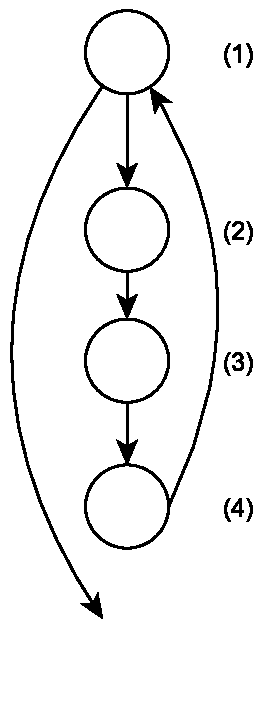
\includegraphics[width=0.85\textwidth,height=0.5\textheight,keepaspectratio]{images/iterative_control_graph}
	\caption{Граф управления для итеративного алгоритма}
	\label{iterative_control_graph}
\end{figure}

На рисунке~\ref{iterative_info_graph} представлен информационный граф, отображающий потоки передачи данных между операторами.

\begin{figure}[H]
	\centering
	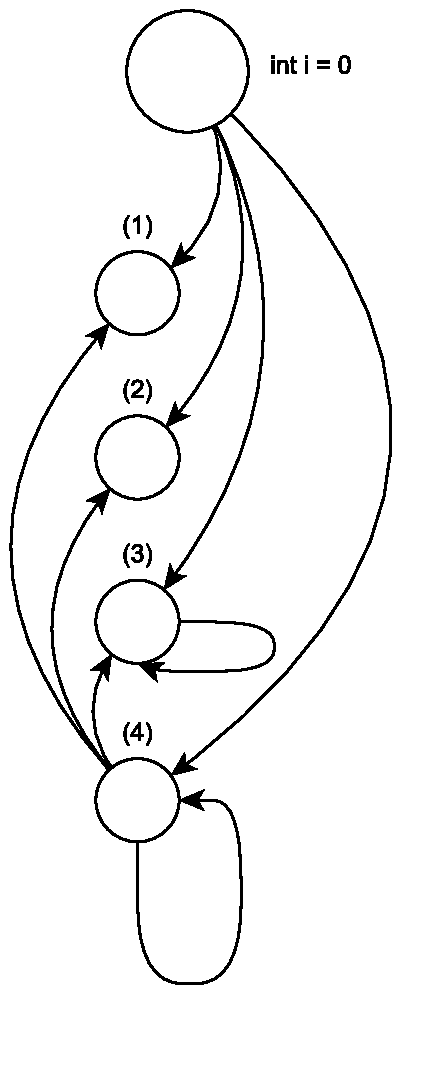
\includegraphics[width=0.85\textwidth,height=0.5\textheight,keepaspectratio]{images/iterative_info_graph}
	\caption{Информационный граф для итеративного алгоритма}
	\label{iterative_info_graph}
\end{figure}

На рисунке~\ref{iterative_oper_history} показан граф операционной истории, где вершины --- срабатывания операторов, а дуги --- последовательность их выполнения.

\begin{figure}[H]
	\centering
	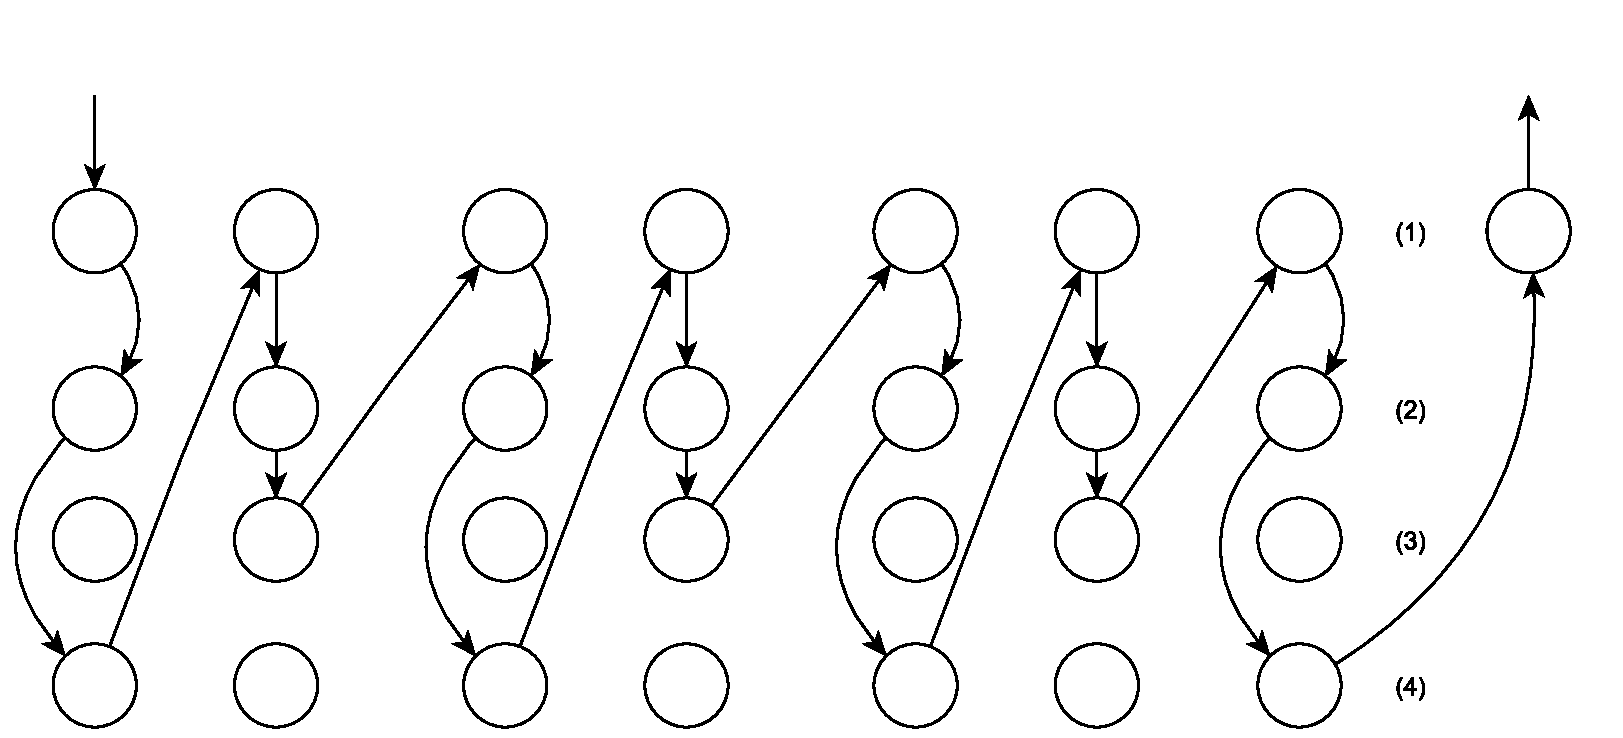
\includegraphics[width=0.85\textwidth,keepaspectratio]{images/iterative_oper_history}
	\caption{Граф операционной истории для итеративного алгоритма}
	\label{iterative_oper_history}
\end{figure}

На рисунке~\ref{iterative_info_history} приведён граф информационной истории, демонстрирующий информационные зависимости между срабатываниями операторов.

\begin{figure}[H]
	\centering
	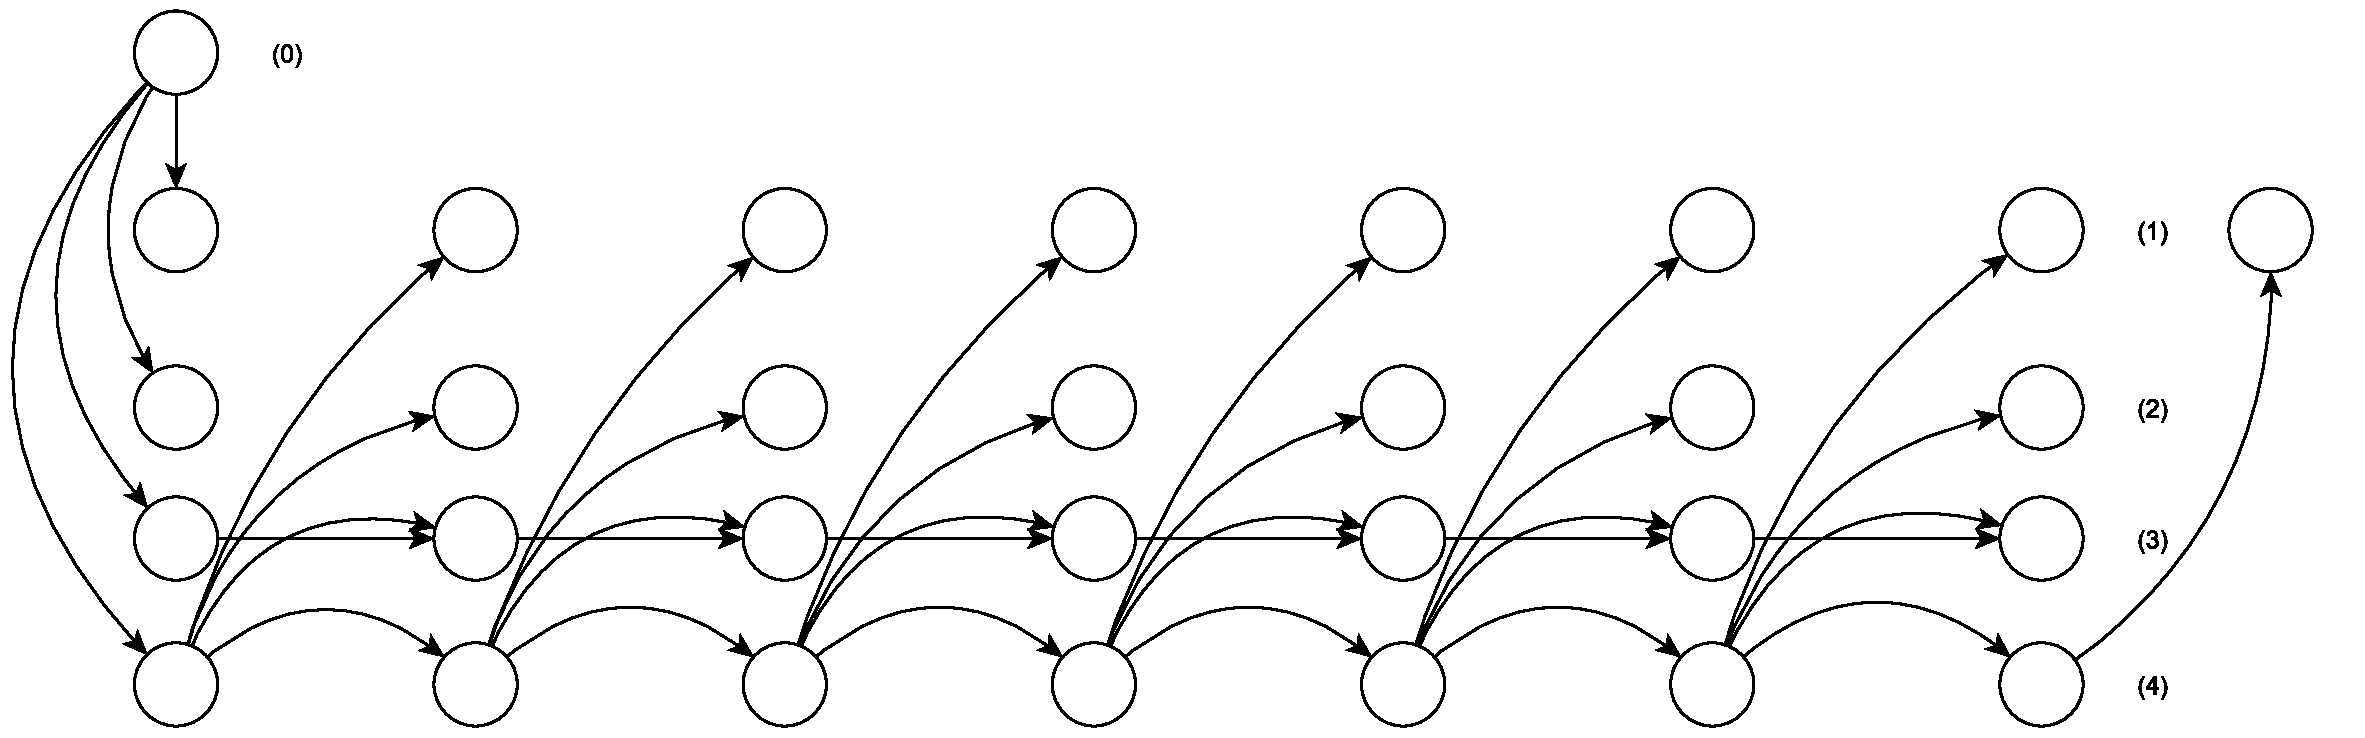
\includegraphics[width=0.85\textwidth,keepaspectratio]{images/iterative_info_history}
	\caption{Граф информационной истории для итеративного алгоритма}
	\label{iterative_info_history}
\end{figure}

\section{Графовые модели рекурсивного алгоритма}

Основные операторы рекурсивного алгоритма:
\begin{enumerate}
	\item проверка конца последовательности: \texttt{if (index >= sequence.size())};
	\item проверка нечётности позиции: \texttt{if ((index + 1) \% 2 != 0)};
	\item вывод текущего элемента: \texttt{std::cout << sequence[index] << " "};
	\item рекурсивный вызов функции: \texttt{printOddPositionsRecursive(sequence, index + 1)}.
\end{enumerate}

\subsection{Графы рекурсивного алгоритма}

На рисунке~\ref{recursive_control_graph} представлен граф управления рекурсивного алгоритма, демонстрирующий порядок выполнения операторов.

\begin{figure}[H]
	\centering
	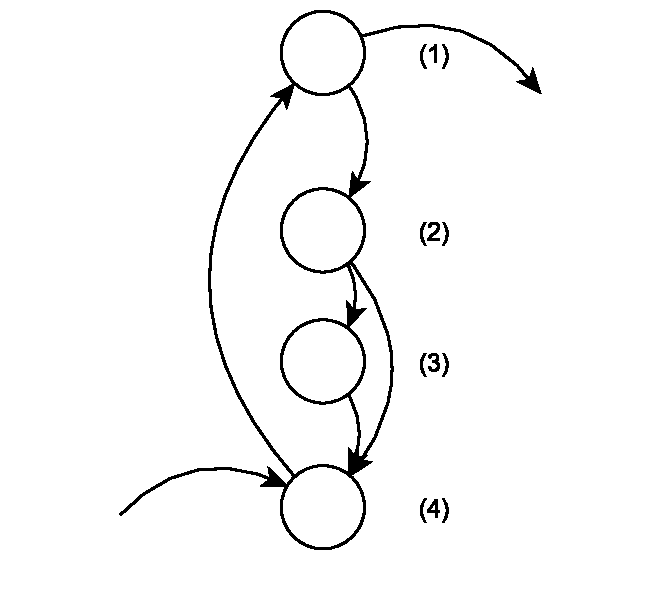
\includegraphics[width=0.85\textwidth,height=0.5\textheight,keepaspectratio]{images/recursive_control_graph}
	\caption{Граф управления для рекурсивного алгоритма}
	\label{recursive_control_graph}
\end{figure}

На рисунке~\ref{recursive_info_graph} приведён информационный граф, отображающий потоки данных между операторами.

\begin{figure}[H]
	\centering
	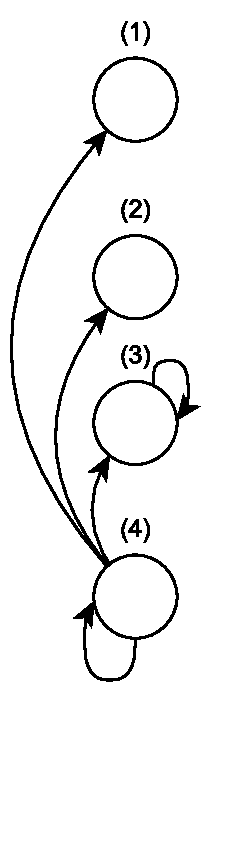
\includegraphics[width=0.85\textwidth,height=0.5\textheight,keepaspectratio]{images/recursive_info_graph}
	\caption{Информационный граф для рекурсивного алгоритма}
	\label{recursive_info_graph}
\end{figure}

На рисунке~\ref{recursive_oper_history} показан граф операционной истории, где вершины --- срабатывания операторов, а дуги --- последовательность их выполнения.

\begin{figure}[H]
	\centering
	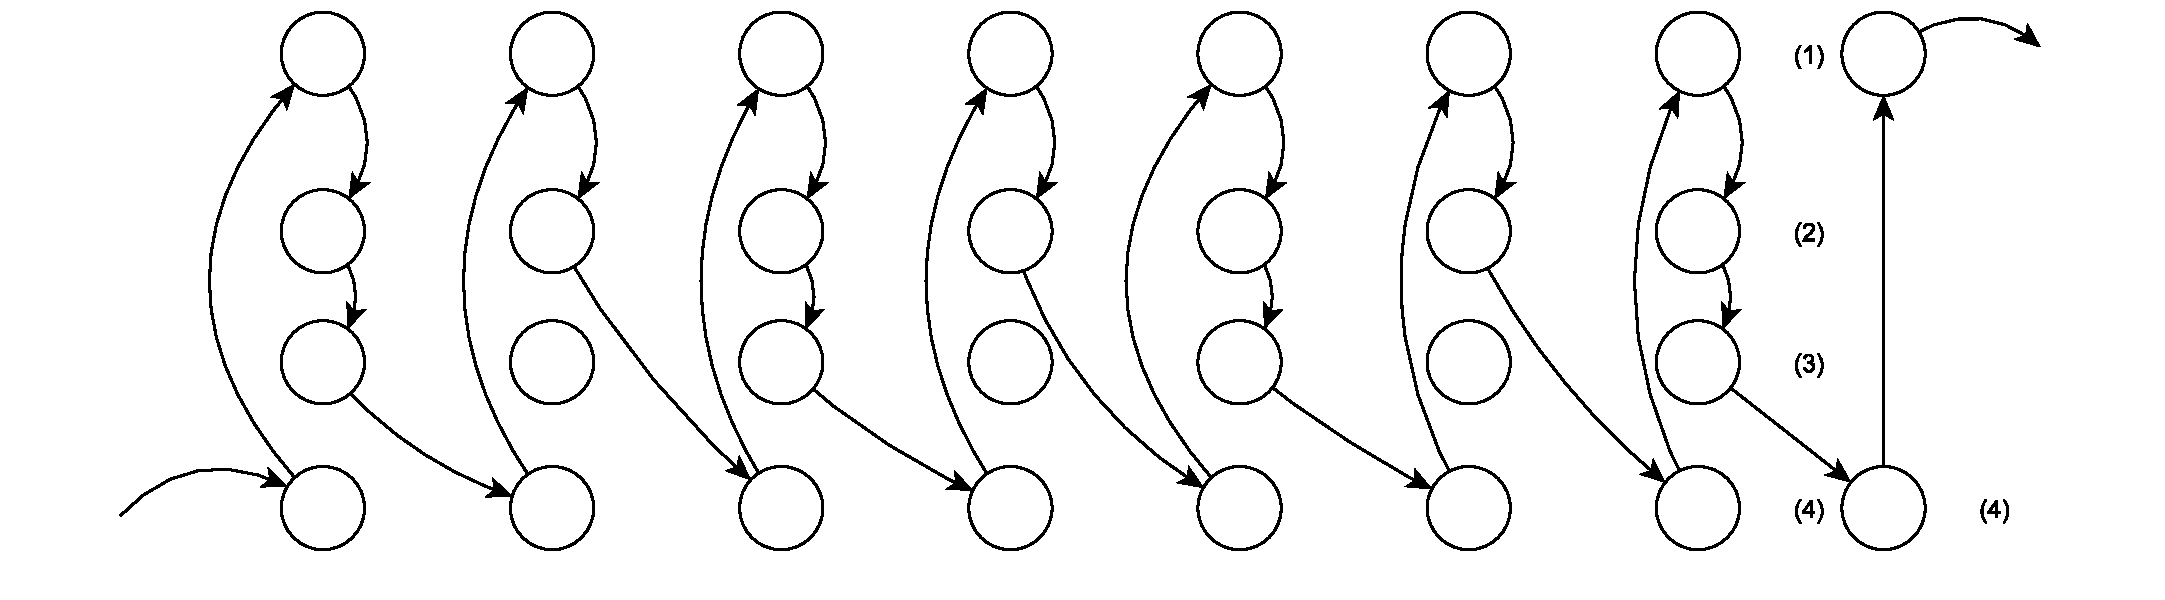
\includegraphics[width=0.85\textwidth,keepaspectratio]{images/recursive_oper_history}
	\caption{Граф операционной истории для рекурсивного алгоритма}
	\label{recursive_oper_history}
\end{figure}

На рисунке~\ref{recursive_info_history} изображён граф информационной истории, демонстрирующий информационные зависимости между срабатываниями операторов.

\begin{figure}[H]
	\centering
	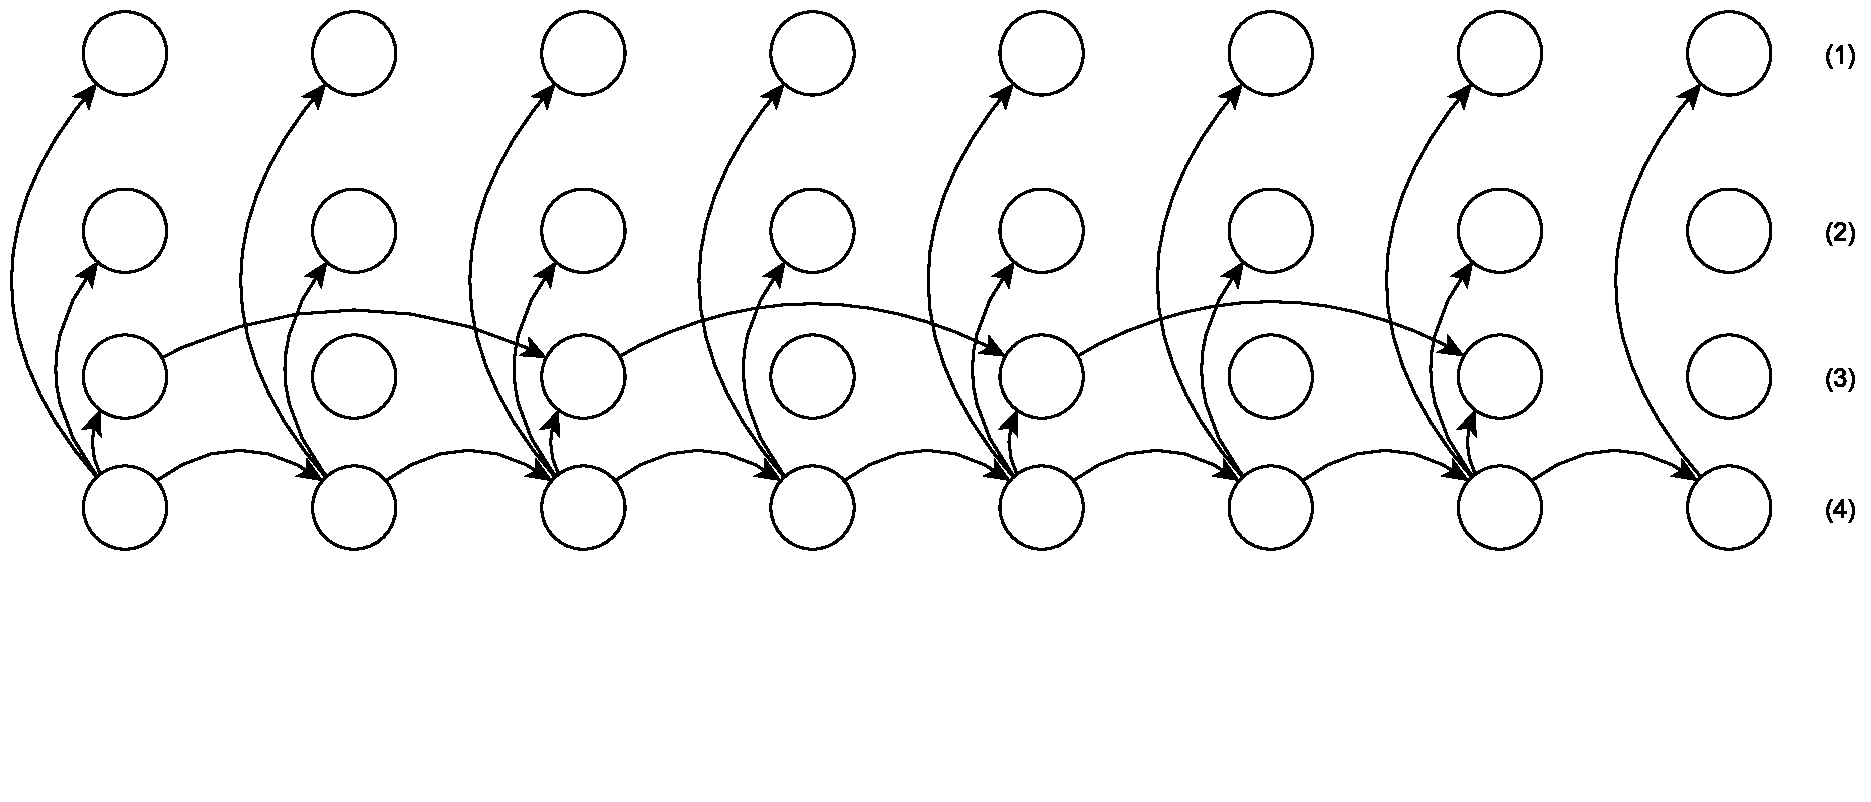
\includegraphics[width=0.85\textwidth,keepaspectratio]{images/recursive_info_history}
	\caption{Граф информационной истории для рекурсивного алгоритма}
	\label{recursive_info_history}
\end{figure}

\section*{Вывод}

Анализ графовых моделей показал, что оба алгоритма выполняются последовательно: каждая операция зависит от предыдущей, что исключает возможность распараллеливания.  
Различие состоит только в организации вычислений: рекурсивный алгоритм использует стек вызовов, итеративный --- цикл.
